%
% dipol1.tex -- Situation beim 1-dimensionalen Dipol
%
% (c) 2017 Prof Dr Andreas Müller, Hochschule Rapperswil
%
\documentclass[tikz]{standalone}
\usepackage{times}
\usepackage{txfonts}
\usepackage{fp}
\usepackage{ifthen}
\usepackage[utf8]{inputenc}
\usetikzlibrary{arrows,intersections}
\usetikzlibrary{fixedpointarithmetic}
\begin{document}
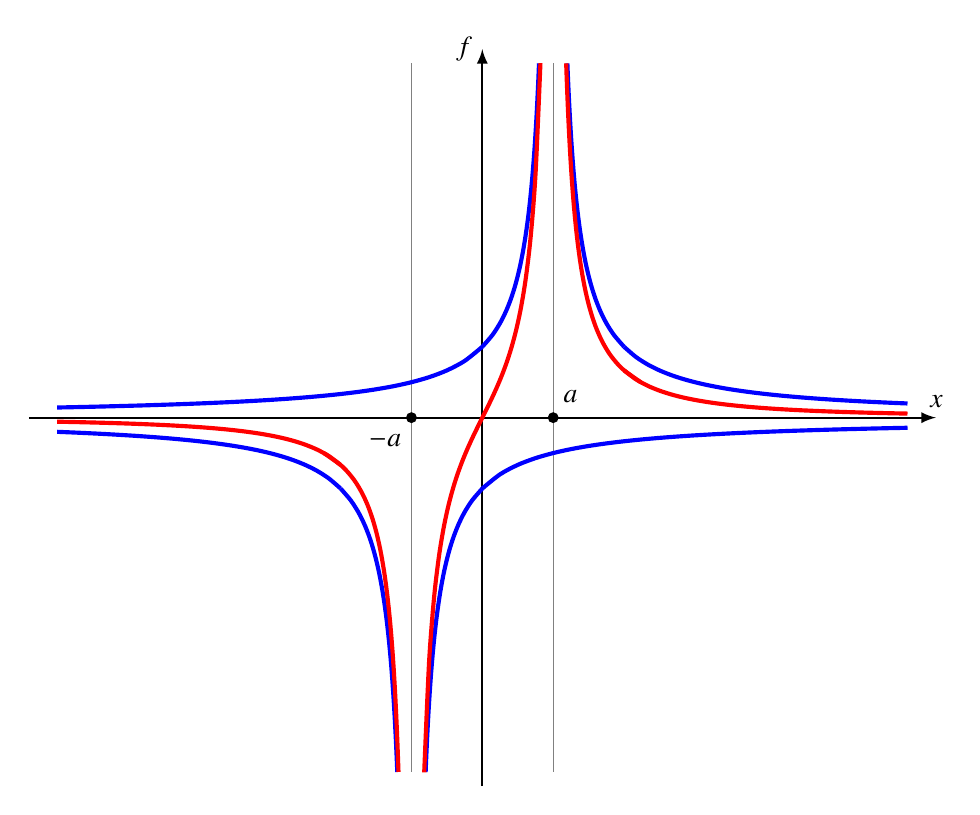
\begin{tikzpicture}[>=latex, thick, scale=1.8]

\draw[color=gray,line width=0.5] (-0.5,-2.5)--(-0.5,2.5);
\draw[color=gray,line width=0.5] ( 0.5,-2.5)--( 0.5,2.5);

\draw[->] (-3.2,0)--(3.2,0) coordinate[label={above:$x$}];
\draw[->] (0,-2.6)--(0,2.6) coordinate[label={left:$f$}];

\draw[fill=black] (-0.5,0) circle[radius=0.3mm,fill]{};
\draw[fill=black] (+0.5,0) circle[radius=0.3mm,fill]{};

\node at (-0.5,0) [below left] {$-a\mathstrut$};
\node at ( 0.5,0) [above right] {$\mathstrut a$};

\draw[line width=1.5,scale=0.5,domain=2:6,smooth,variable=\x,blue]
	plot ({\x},{1/(\x-1)});
\draw[line width=1.5,scale=0.5,domain=2:8,smooth,variable=\x,blue]
	plot ({2-\x},{1/(\x-1)});
\draw[line width=1.5,scale=0.5,domain=1:5,smooth,variable=\y,blue]
	plot ({1 + 1/\y},{\y});
\draw[line width=1.5,scale=0.5,domain=1:5,smooth,variable=\y,blue]
	plot ({1 - 1/\y},{\y});

\draw[line width=1.5,scale=0.5,domain=0:6,smooth,variable=\x,blue]
	plot ({\x},{-1/(\x+1)});
\draw[line width=1.5,scale=0.5,domain=0:4,smooth,variable=\x,blue]
	plot ({-2-\x},{-1/(\x+1)});
\draw[line width=1.5,scale=0.5,domain=1:5,smooth,variable=\y,blue]
	plot ({-1 + 1/\y},{-\y});
\draw[line width=1.5,scale=0.5,domain=1:5,smooth,variable=\y,blue]
	plot ({-1 - 1/\y},{-\y});

\draw[scale=0.5,domain=2:6,smooth,variable=\x,red,line width=1.5]
	plot ({\x}, {1/(\x-1) - 1/(\x+1)});
\draw[scale=0.5,domain=0.5:5,smooth,variable=\y,red,line width=1.5]
	plot ({sqrt(1+2/\y)}, {\y});

\draw[scale=0.5,domain=2:6,smooth,variable=\x,red,line width=1.5]
	plot ({-\x}, {-1/(\x-1) + 1/(\x+1)});
\draw[scale=0.5,domain=0.5:5,smooth,variable=\y,red,line width=1.5]
	plot ({-sqrt(1+2/\y)}, {-\y});

\draw[scale=0.5,domain=-0.82:0.82,smooth,variable=\x,red,line width=1.5]
	plot ({\x},{-1/(\x+1) - 1/(\x-1)});

\end{tikzpicture}
\end{document}
